\chapter{Performance Evaluation of ALOHA in context of multiple Base Station}

% **************************** Define Graphics Path **************************
\ifpdf
    \graphicspath{{Chapter3/Figs/Raster/}{Chapter3/Figures/PDF/}{Chapter3/Figures/}}
\else
    \graphicspath{{Chapter3/Figs/Vector/}{Chapter3/Figures/}}
\fi

\section{Introduction}
%Machine Type Communication (MTC) is characterized by a large number of terminals, small payload and uplink-centric.
Machine Type Communication (MTC) is expected to gain more popularity in the next decade, which poses great challenges for traditional wireless networks: long range coverage,  low power consumption, access network overload, etc. To tackle with the brought problems,
there are two types of long range MTC systems to handle MTC traffic:\begin{inparaenum}[1)]
 	\item MTC-dedicated networks, also called Low Power Wide Area Network (LPWAN);
 	\item existing cellular networks with adaptations, such as NB-IoT networks~\cite{goursaud2015dedicated}\cite{song2016survey}.
 \end{inparaenum}
For both types of networks, ALOHA plays an important role: either as an initial access method to send a request packet to get resource in cellular networks, or as a data packet transmission method in LPWAN. 
%The MTC-dedicated wireless networks are more attractive faced with MTC specific features~\cite{goursaud2015dedicated}. 

In cellular networks, the packet is sent in unicast mode: the destination Base Station (BS) is indicated by the terminal. However, it also could be sent in broadcast mode, and benefit from macro reception diversity, which is defined as the capacity of several BS to receive the same packet. As for BS, there exist two possibilities to process the received packets. The first one is that each BS autonomously demodulates and decodes the packets (see Fig.~\ref{fig:macro_diversity_recpetion_illustration}). The core network is in charge of duplicate received packets removal (e.g., by comparing the identity and message content conveyed in packets). Such a scheme is presently applied by some LPWAN networks, such as SigFox and LoRaWAN~\cite{ietf-lpwan-overview-03}. The second possibility is that signals received at each BS are linearly combined in the core network so that the output SINR is maximized (see Fig.~\ref{fig:mrc_macro_diversity_recpetion_illustration}). This scheme is like the well-known maximum ratio combining (MRC) technique in Multiple-Input Multiple-Output (MIMO) systems\qsong{Christophe Fourtet said that they were working on combining scheme. I think it's important to give a reference here}. The processing in the core network in both case is out of the scope of this thesis. 
Due to the broadcast nature, the BSs in networks enabling macro reception diversity do not acknowledge the received packets. Hence, the device has to repeat each packet transmission fixed times at random time interval, even if one previous trial is successful. If none of these trials is successful. the packet is lost and the device has no awareness about this.

Not surprisingly, macro reception diversity outperforms the traditional unicast mode in terms of one-shot random access packet loss rate, which means higher system capacity constrained by packet loss rate. However, unicast mode can use retransmission mechanism to reduce packet loss rate while message repeat in macro reception diversity reduces its throughput. The capacity of each mode, which is the maximum supported load for a given packet loss rate target is derived. The ratio between the two capacity values is called the \emph{macro diversity gain}. In this chapter, we give a thorough performance comparison between these two modes, in terms of packet loss rate\qsong{We should use a better metric other than the simple averaged packet loss rate over infinite plane.} , macro diversity gain, throughput\qsong{maybe can consider other metrics...}. We first consider the one-shot random access case and then extend with retransmission mechanism.\qsong{How to include/organize the case of known nearest BS...It's a question...}

%Thus, devices in such networks transmit packets in a ``broadcast`` manner without attach procedure used in cellular networks. SigFox is an example applying the aforementioned macro reception diversity. 
\begin{figure}[!ht]
	\centering
	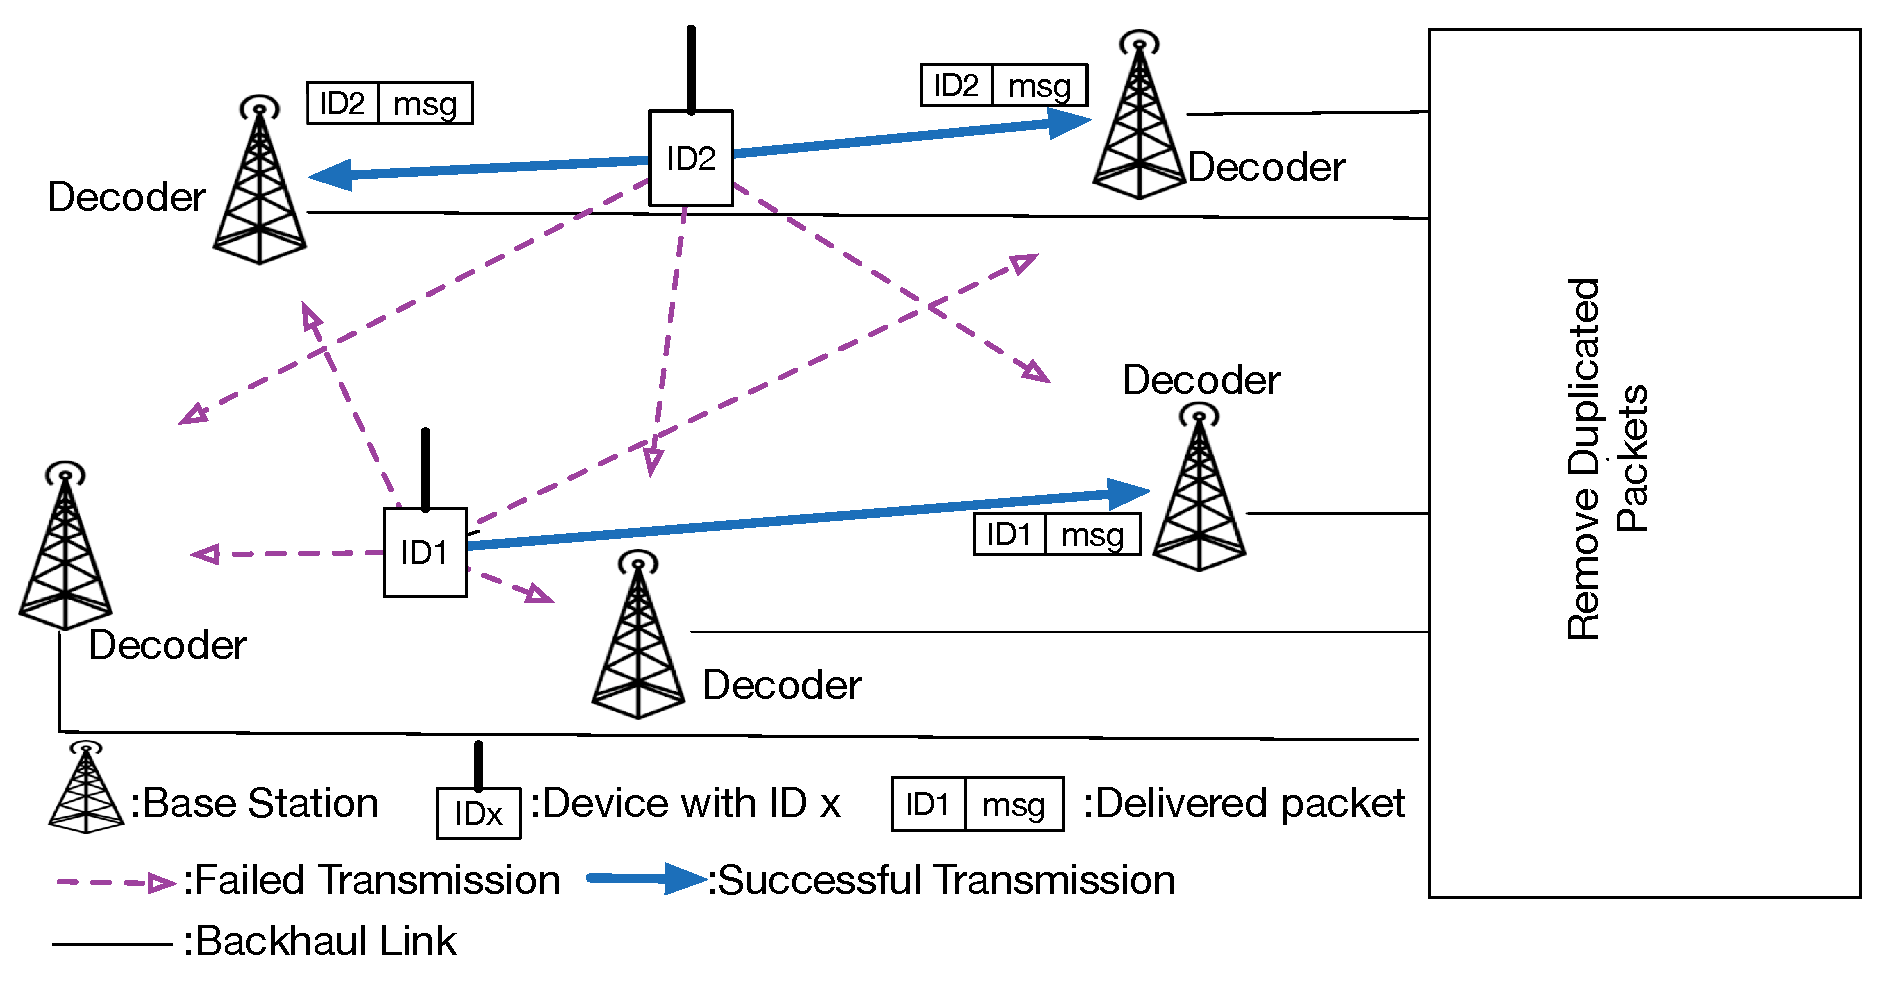
\includegraphics[width=\linewidth]{Chapter5/Figures/Macro_Diversity_Recpetion_Illustration}
	\caption{Macro Reception Diversity Scheme Illustration\qsong{Since we call Maximum Ratio Combining Macro Reception Diversity in anther figure, I'm not sure we should modify the caption of this figure as Selective Combining-like Macro Diversity Reception. Because it is equivalent to judge whether the maximum SINR is greater than captio ratio...}}
	\label{fig:macro_diversity_recpetion_illustration}
\end{figure} 

\begin{figure}[!ht]
	\centering
	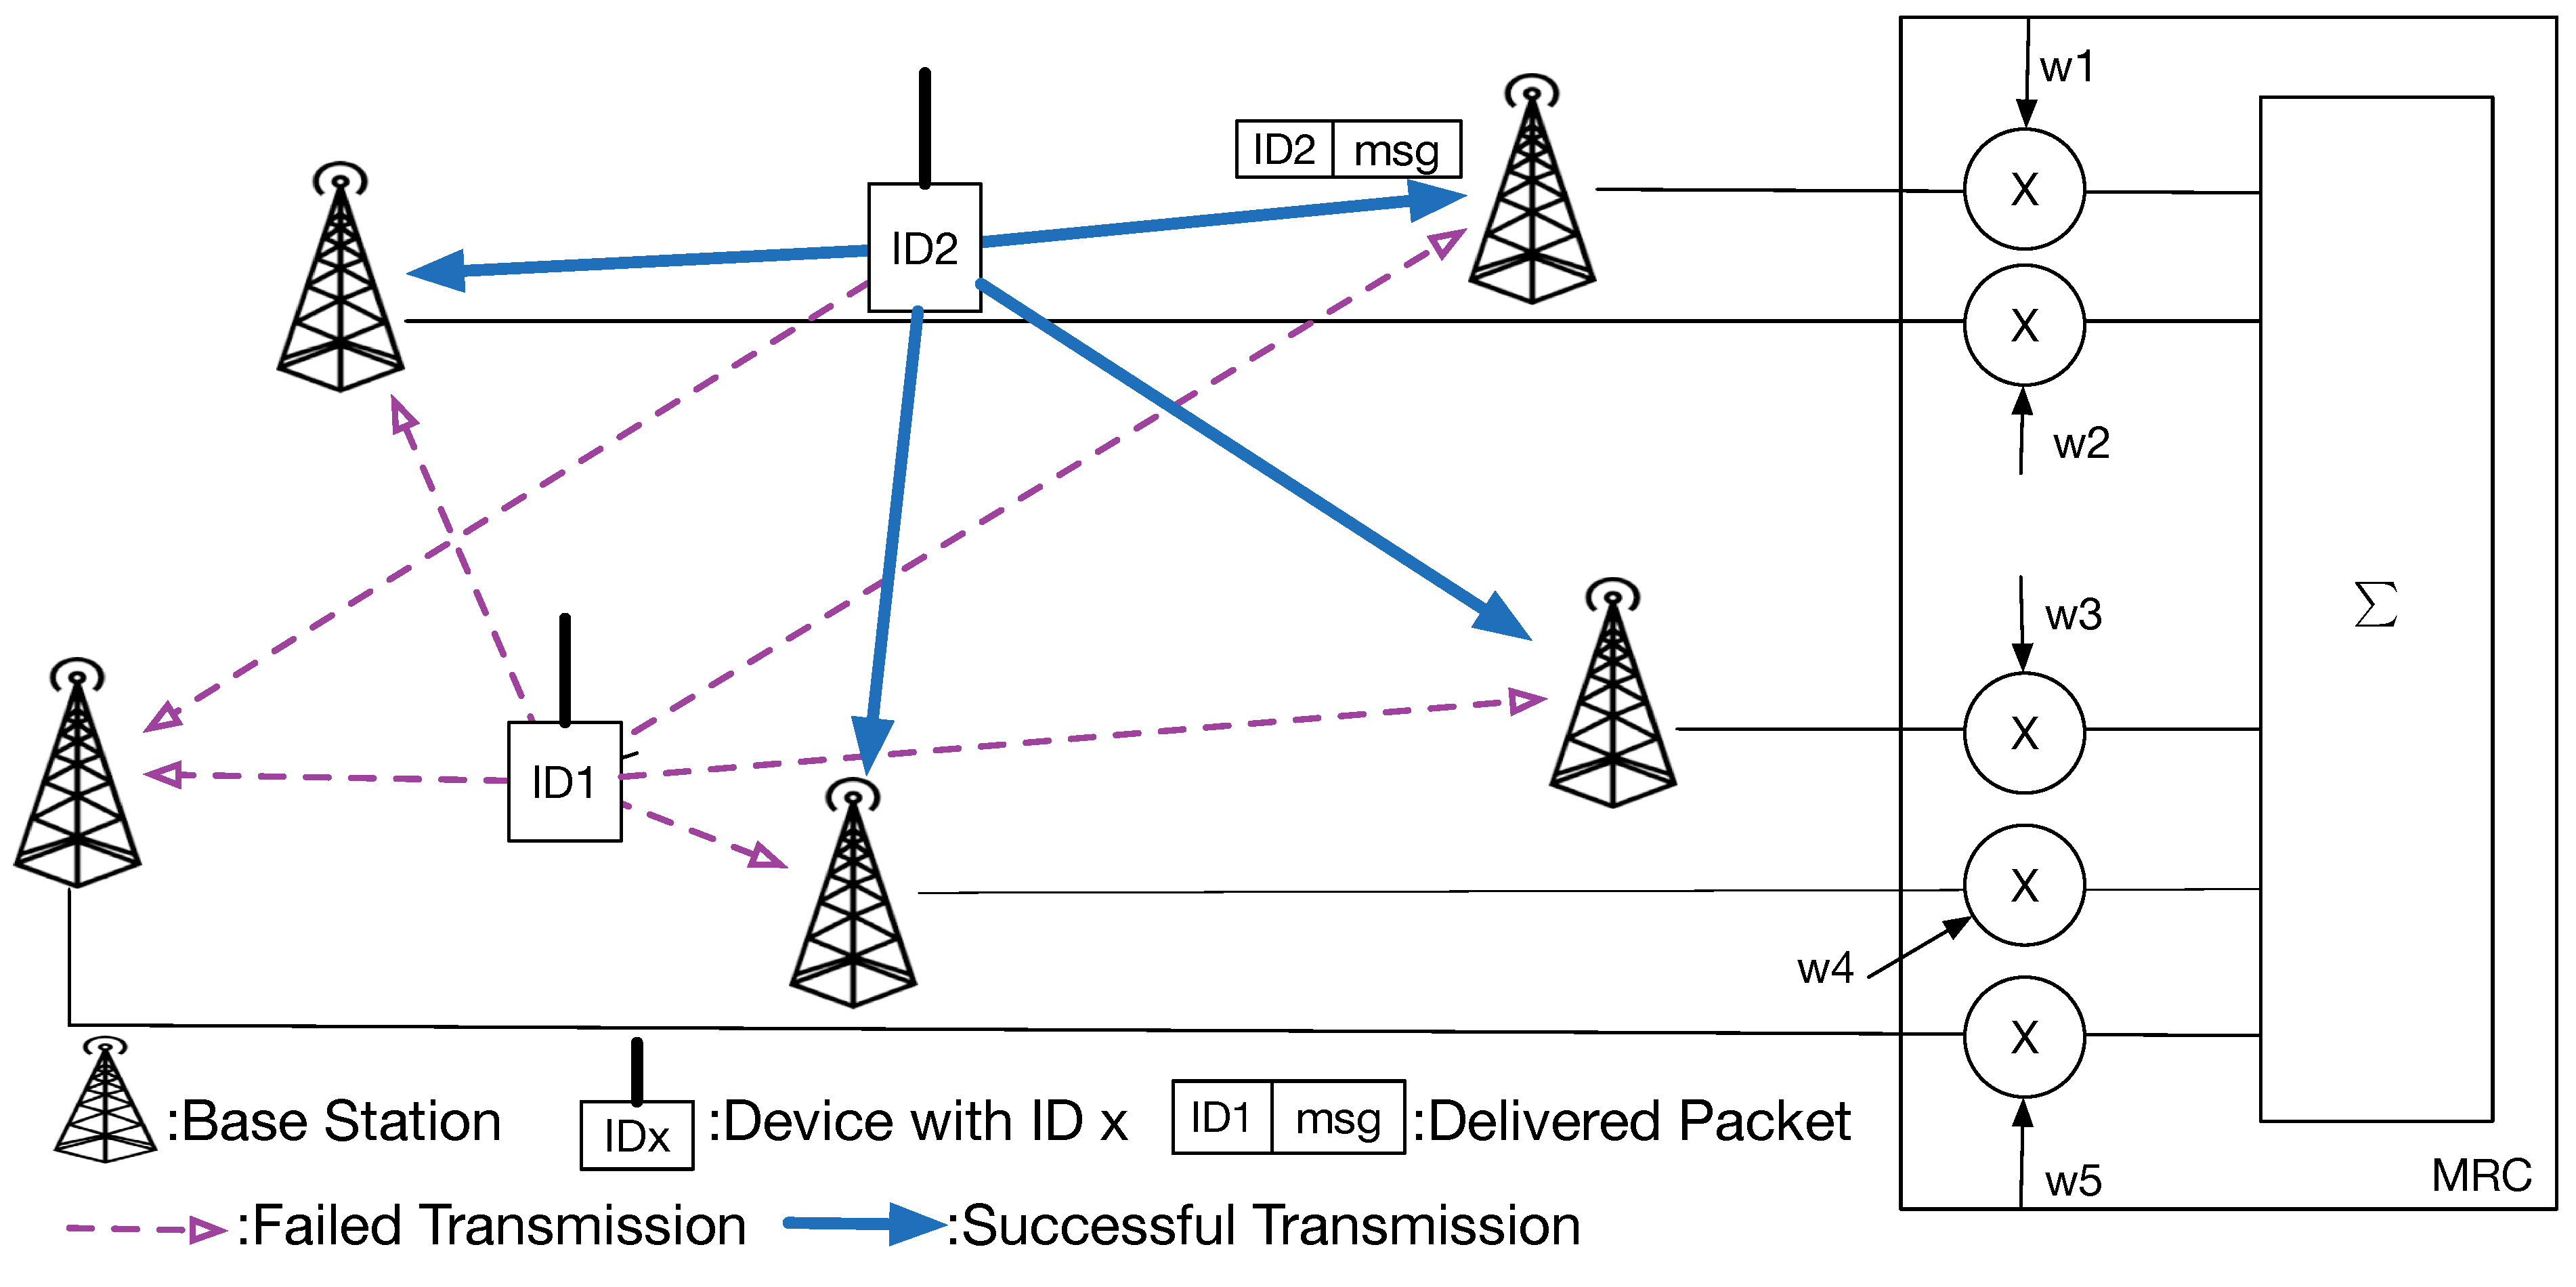
\includegraphics[width=\linewidth]{Chapter5/Figures/MRC_Type_Macro_Diversity_Recpetion_Illustration}
	\caption{Maximum Ratio Combining Macro Reception Diversity Scheme Illustration. The coefficients $w1, w2, ..., w5$ are well designed so that output SINR is maximized.}
	\label{fig:mrc_macro_diversity_recpetion_illustration}
\end{figure} 
%In this broadcast mode, the BSs do not acknowledge the received packets. Hence, the device has to repeat each packet transmission fixed times at random time interval, even if one previous trial is successful. If none of these trials is successful. the packet is lost and the device has no awareness about this. Such a scheme is presently applied by some low-cost dedicated IoT networks, such as SigFox. 

%Not surprisingly, macro reception diversity outperforms the traditional unicast mode in terms of one-shot random access packet loss rate, which means higher system capacity constrained by packet loss rate. However, unicast mode can use retransmission mechanism to reduce packet loss rate while message repeat in macro reception diversity reduces its throughput. 

%In this letter, we propose a simple but accurate analytical model for pure (i.e. non-slotted) and slotted ALOHA based on available stochastic geometry research results. The proposed model takes into account Rayleigh fading, shadowing and capture effect in wireless channel. One can use this model to quantify the macro reception diversity gain in terms of maximum supported load constrained by packet loss rate. 

%derive how many times devices macro reception diversity can serve more that the unicast mode, in a commonly agreed system model. We call the latter performance metric as macro diversity gain.
\section{State of the Art
% TODO: the related work part is not enough detailed. To be detailed afterwards.
%	\qsong{to be detailed...}
}
In literature, the performance of ALOHA-based LPWAN are usually analyzed with Stochastic geometry. Baccelli et al.~\cite{baccelli2006aloha} use Laplace transform for interference analysis for slotted ALOHA. Haenggi et al.~\cite{haenggi2009interference} extensively study the outage probability in SINR-based capture model for slotted ALOHA. B{\l}aszczyszyn et al.~\cite{blaszczyszyn2010stochastic} open the door to study pure ALOHA with stochastic geometry. However, to our best knowledge, macro reception diversity for ALOHA systems has not been studied in literature.
\section{System model}
\label{sec:system_model}
% Xavier's suggestion:
%	Plus précisément, ce qui me semble intéressant c'est de comprendre l'évolution des performances pour 3 configurations
%- Slotted Aloha avec transmission à la meilleure BS et avec une voie de retour (type réseau cellulaire)
%- Pure Aloha avec macro-diversité et une voie de retour (type LORA)
%- Pure Aloha avec macro-diversité sans voie de retour (type LORA)
\subsection{Distribution of Nodes and Traffic Model}
We consider a large wireless network over a two-dimension infinite plane. The locations of terminals form a stationary Poisson point process (PPP) $\Phi_m = \left\lbrace X_i\right\rbrace$ on the plane $\mathbb{R}^2$ with spatial density $\lambda_m$.  Similarly, the locations of base stations also form a stationary PPP $\Phi_b = \left\lbrace Y_i\right\rbrace$ with spatial density $\lambda_b$. One devices and BSs spatial distribution realization is shown in Fig.~\ref{fig:device_BS_spatial_distribution}. All the packets transmitted by devices have the same duration $B$.
\begin{figure}[!ht]
	\centering
	\includegraphics[width=\linewidth]{/Users/qsong/Documents/slotted_aloha_related_project/multiple_recepteur_capacity/nodes_spatial_dist.eps}
	\caption{Maximum Ratio Combining Macro Reception Diversity Scheme Illustration. The coefficients $w1, w2, ..., w5$ are well designed so that output SINR is maximized.}
	\label{fig:device_BS_spatial_distribution}
\end{figure} 

\subsection{Slotted ALOHA and Pure ALOHA}
For a comparison between macro reception diversity and traditional BS attach method, we consider three types of ALOHA-based network. As a comparison reference, we consider a traditional cellular network which employs slotted ALOHA. The devices in such a network attach to its best BS for which the received power averaged over all fading realizations is the strongest. For macro reception diversity, it is assumed to run in pure slotted ALOHA. Furthermore, this networks with macro reception diversity can be divided into two categories: with downlink for acknowledgment (e.g. LoRaWAN) and without downlink for acknowledgment (note that SigFox has downlink support but does not use it for acknowledgment). Note that whether acknowledgment is supported has an impact on retransmission mechanism. 

For slotted ALOHA, the time domain is equally divided into slots with duration $B$. In each slot, each device independently decides to transmit a packet with probability $p$. The propagation delay is assumed to be much smaller than $B$. Hence, there is a global slot synchronization over the whole network.

In pure ALOHA, devices send packets without synchronization, but we still use parameter $p$. The packet generation process can be seen as an internal slotted system in each device with $p$ the probability to transmit in a slot of duration $B$.

At a given time, the locations of terminals that are transmitting a packet form a PPP with spatial density $p\lambda_{m}$. For slotted and pure ALOHA, we define the normalized load (per BS) as $L = p\lambda_{m}/\lambda_{b}$. In addition, we just consider one-shot random access. This model can be easily extended with retransmission mechanisms.
\subsection{Random Channel and Capture Effect}
% Xavier insists that this is a communication letter which should be concise.
% Not necessary to explain somethings well-known for readers with enough background knowledges.
We assume that M2M devices do not support power control mechanism due to the low-cost constraint and transmit with unit power level. M2M-dedicated networks are usually narrow band and thus can be assumed to suffer Rayleigh fading. For example, NB-IoT use $180$ kHz bandwidth~\cite{wang2017primer} and SigFox's bandwidth is $100$ Hz~\cite{raza2017low}. The bandwidth of $LoRaWAN$ varies from $125$ kHz to $500$ kHz according to different spread-spectrum sequence. Although LoRaWAN applies spectrum spreading technology, it can still be assumed to suffer Rayleigh fading~\cite{georgiou2017low} in literature.
Thus, the received power $P_{r}$ of a packet at the base station side depends on path-loss attenuation $r^{-\gamma}$, Rayleigh fading $H$ and shadowing effect $\exp(\chi)$:
\begin{align}
\label{eq:path-loss}
P_{r} =d^{-\gamma} H \exp(\chi),
\end{align}
%The path-loss attenuation $l(r)$ is defined as $l(r) = r^{-\gamma}$, 
where $d$ refers to the distance between the transmitter and the receiver, $\gamma$ is the path-loss exponent, $H$ is an exponentially distributed random variable (r.v.) with unit mean, $\chi$ is a zero-mean Gaussian r.v. with variance $\sigma^2$. Log-normal shadowing is usually characterized in terms of its dB-spread with standard deviation $\sigma_{dB} = \frac{10}{\ln(10)}\sigma$. We assume that $H$ and $\chi$ are both constant during a packet transmission, and mutually independent for different links. 
%Due to channel randomness, it is possible that the received power at a far device is stronger than a close device. 

\subsection{Displacement theorem and transformed PPP}
\label{subsec:displacement_theorem}
As mentioned in Sec.~\ref{sec:system_model}, each device is assumed to connect to the BS that provides the highest long-term biased received power. The inclusion of shadowing allows to rewrite $\eqref{eq:path-loss}$ as follows:
\begin{align}
P_{r} 
&= H \left[  \exp^{-1/\gamma}(\chi) d \right]  ^ {-\gamma},
\end{align}
where shadowing can be interpreted as a random displacement of the location of BS. This fact can be leveraged by using displacement theorem~\cite{franccois2009stochastic}. That is to say, attaching to the best BS in a PPP of intensity $\lambda_{b}$ with shadowing is equivalent to attaching the geographically nearest one in a transformed PPP of intensity $\lambda_{b} \mathbb{E}\left[ e^{-\frac{2}{\gamma}\chi}\right] = \lambda_{b} e^{\frac{2\sigma^2}{\gamma^2}}$ without shadowing. This lemma is given in~\cite[lemma 1]{dhillon2014downlink} and detailed proof is given in~\cite[Corollary 3]{madhusudhanan2014downlink}. We use $r$ to denote the distance between device and BS in the transformed PPP.

%Capture effect refers to the fact that signals in collision can still be demodulated if their received SINR are greater than or equal to a certain threshold value. 
Capture effect is taken into account in the proposed model. Thus, the transmission success probability $p_{s}$ for a transmit-receiver pair is defined as follows: 
\begin{align}
\label{eq: sinr-definition}
p_s = \mathbb{P}\left\lbrace  \text{SINR} = \frac{P_r}{I + N} \geq \theta_{T} \right\rbrace, 
\end{align}
where $I$ refers to the suffered cumulative interference during packet transmission, $N$ is the normalized background noise power. It is worthwhile to mention that in some cases the background noise is rationally negligible for the sake of tractability.

\subsection{Impact of background noise}
Actually, the background noise is usually neglected in the study of LPWAN system. One institutive exposition about this is that the occupied transmission bandwidth is small and the noise power is at a low level. Here, we give an estimation about the normalized noise power value $N$ if transmit power is assumed to be $1$. To this end, we have to know, in a realistic LPWAN network, the ratio between the received power and the real background noise level.

For one LPWAN device running on ISM band (e.g. with 868 MHz), from a regulatory point of view, the effective radiated power (ERP) may not exceed $14$ dBm (or $25$mW) in any direction, we thus assume that the transmit power is set as $14$ dBm.

About noise power level, we use the same formula given in~\cite{georgiou2017low}:
\begin{align}
	N_{\textbf{real}} = -174 + NF + 10\log(W) ,
\end{align}
where $NF$ is noise figure, usually set as $6$dB, $W$ is the bandwidth occupied by the transmitted packet. The occupied transmission band is assumed to be between $100$ Hz and $200$ KHz. Thus, the possible value of $N_{\text{real}}$ is between $-148$ dBm and $-115$ dBm.

In terms of propagation path-loss model, Okumura-Hata model is applied. In urban area, the path-loss between one device and a BS with height $50$ meters is~\cite{lagrange2000reseaux}:  
\begin{align}
	\text{Path_Loss}= 123.6+33.8\log(d),
\end{align}
where $\log(\cdot)$ is $10$-based logarithm operator.

Therefore, if we assume that transmit power is $1$, the normalized noise power $N$ should take values in range $\left[ -38.4, -5.4\right] $. 
%According to the simulation that we have conducted, 



%\subsection{Performance Metric}
%\subsubsection{Packet loss rate}
%xxx
%\subsubsection{Macro Diversity Gain}
%xxx
%\subsubsection{Throughput}
%xxx
%\subsubsection{Energy efficiency}
%xxx
%Similarly, we also consider two different ways to estimate interference with respect to device coding schemes. If no interleaving and error correction code technique are not used, the cumulative interference is the maximal interference value during the transmission B: $I^{\text{max}} = \max I(t)$ for $t \in \left[ T, T+B\right] $. If advanced techniques to resistant transmission error are used, average interference over the packet transmission $I^{\text{mean}} = \frac{1}{B}\int_{T}^{T+B} I(t)dt$.

%Empirical measurements shows that shadowing effect, when represented in dB units, follows a normal distribution (see e.g.\cite{erceg1999empirically}). In other words, the linear (as opposed to dB) channel gain may be modeled by a log-normal random variable, $e^G$, where $G$ is a zero-mean Gaussian r.v. with variance $\sigma^2$. Log-normal shadowing is usually characterized in terms of its dB-spread, $\sigma_{dB}$, which is related to $\sigma$ by $\sigma = \frac{\ln(10)}{10}  \sigma_{dB}$. Thus, The received power $P_{r}$ is expressed as follows:

%As to the non-slotted ALOHA protocol, we still divide the time domain into slot of length $B$, one packet appears with probability $p$ in a given slot, but the packet arrival time is not the beginning of a slot like in slotted ALOHA. Instead, packet arrival time is uniformly distributed in a slot. 

%At a given time, the locations of terminals that are transmitting a packet form a PPP with spatial density $p\lambda_{m}$. A BS can correctly receive at most one packet at a given time. 
%For slotted and pure ALOHA, we define the normalized load (per BS) as $p\lambda_{m}/\lambda_{b}$. In non-overload conditions, $p\lambda_{m}/\lambda_{b} < 1$.













\section{Link-level Transmission Success Probability}
\label{sec:trans_succ_p_pair}
We first study the transmission success probability $p_s(r)$ for a given uplink between a BS at the origin and a device $x_0$ at distance $r$. Using Slivnyak's theorem~\cite{vaze2015random}[Theorem 2.3.3], combining $(\ref{eq:path-loss})$ and $(\ref{eq: sinr-definition})$, we have:
\begin{align}
p_{s} \left( r\right)
& =\mathbb{P}\left\lbrace \frac{H \exp(\chi) r^{-\gamma}}{\sum_{x_j \in \Phi_{m}} H_{x_j} \exp(\chi_{x_j}) r_{x_j}^{-\gamma}}  \geq \theta_T \right\rbrace. \nonumber
\end{align}
Let $I=\sum_{x_j \in \Phi_{m}} H_{x_j} \exp(\chi_{x_j}) r_{x_j}^{-\gamma}$, which is the cumulative interference suffered by $x_0$. Conditioned on log-normal shadowing component $\exp(\chi_{x_j}) $, as shown in~\cite{haenggi2009interference}, $p_{s}\left( r \right)$ can be expressed in terms of Laplace transform of cumulative interference $\mathcal{L}_{I}(s)$ at point $\theta_{T} e^{-\chi} r^{\gamma}$:
\begin{align}
\label{eq:def_ps}
p_{s}\left( r \right)  &= Pr \left\lbrace H  \geq I \theta_{T} e^{-\chi}r ^{\gamma}  \right\rbrace \nonumber\\ 
% The follwing line can be hidden, not necessary in FINAL_VERSION
%&=\mathbb{E}_{\chi}\left\lbrace  \mathbb{E}_{I} \left[ \exp(-\theta_{T} \exp(-g) r^{\gamma}  I ) \vert \chi = g\right]\right\rbrace   \nonumber\\
&= \int_{-\infty}^{+\infty} \left[ \int_{0}^{+\infty} \exp(-y \theta_{T} e^{-x} r^{\gamma} ) f_{I}(y)dy\right] f_{\chi}(x) dx  \nonumber\\
&= \mathbb{E}_{\chi} \left[ \mathcal{L}_{I}\left\lbrace \theta_{T} e^{-\chi} r^{\gamma}\right\rbrace \right],
\end{align}
where $f_{X} (x)$ is probability density function (PDF) of r.v. $X$, $\mathbb{E}_{X} \left[ \cdot \right] $ is the expectation operator with respect to $X$.
\subsection{Slotted ALOHA}
In slotted ALOHA, the cumulative interference is constant during each slot. The geometry-aware interference analysis for slotted ALOHA is well investigated. Reference~\cite{haenggi2009interference} gives a closed-form expression about the Laplace transform of cumulative interference. With independent Rayleigh fading and log-normal shadowing, we have:
\begin{align}
\label{eq:lp_tr_slotted}
%\mathcal{L}_{I}\left( s \right) &=\exp\left\lbrace -p\lambda_m K_{\text{slotted}} \mathbb{E}\left[ H^{\frac{2}{\gamma}}\exp(\frac{2}{\gamma}\chi)\right]s^{\frac{2}{\gamma}}  \right\rbrace
\mathcal{L}_{I}\left( s \right)  &=\exp \left\lbrace
-p\lambda_m \pi A  \exp \left( 2\sigma^2/\gamma^2\right) s^{2/\gamma}  
\right\rbrace,
\end{align}
where $A = \Gamma(1-\frac{2}{\gamma})\Gamma(1+\frac{2}{\gamma})$ and $\Gamma(z)=\int_{0}^{+\infty} x^{z-1} e^{-x} dx$. 
%is called the spatial contention factor~\cite{haenggi2009outage}, $\Gamma(z)$ is the gamma function defined as $\Gamma(z)=\int_{0}^{+\infty} x^{z-1} e^{-x} dx$. 
%Since $H$ and $\chi$ are independent, $\mathbb{E}\left[ H^{\frac{2}{\gamma}}\exp(\frac{2}{\gamma}\chi)\right] = \Gamma(1+\frac{2}{\gamma}) \exp \left( \frac{\sqrt{2}\sigma}{\gamma}\right) ^2$.
\subsection{Pure ALOHA}
\label{subsec: pure-aloha}
In pure ALOHA, the cumulative interference $I(t)$ suffered by a given packet transmitted in interval $\left[ T, T+B\right]$ is variable during the packet transmission. When advanced transmission techniques (e.g., interleaving, robust channel coding, etc.) are used, $p_{s}(r)$ is a function of the average interference $I^{\text{mean}} = \frac{1}{B}\int_{T}^{T+B} I(t)dt$, which replaces $I$ in $(\ref{eq: sinr-definition})$.

B{\l}aszczyszyn et al. propose a Poisson-rain model~\cite[Sec.2.4]{blaszczyszyn2015interference} that approximates well this case and allows to compute the cumulative interference. They prove that formula $(\ref{eq:lp_tr_slotted})$ can be reused by letting $A=\frac{2\gamma}{\gamma + 2} \Gamma(1-\frac{2}{\gamma})\Gamma(1+\frac{2}{\gamma})$.
%\subsection{Pure ALOHA, maximum interference}

Another case of pure ALOHA is assumed to have no error correction neither interleaving techniques for the purpose of reducing the device-side cost. In this case, the packet is delivered if and only if each bit is correctly received. Hence, the SINR should be larger than or equal to $\theta_{T}$ during $B$. Hence, $p_{s}$ is a function of maximum interference $I^{\text{max}} = \max_{t \in \left[ T, T+B\right]} I(t)$. According to~\cite[Sec.2.4]{blaszczyszyn2015interference}, there is no closed-form for $I^{\text{max}} $, and the authors use a simulation approach to study. Next, we propose a simple upper bound to estimate $I^{\text{max}}$. Section~\ref{sec:simulation} shows that the bias is at an acceptable level.

Consider a packet transmitted in interval $\left[ T, T+B\right]$. Any device generating its interference at $T$ terminates packet transmission before $T+B$. The interfering packets at $T+B$ do not exist at $T$, because the packet transmission duration is $B$. 
Hence, cumulative interference $I(T)$ and $I(T+B)$ are two independent and identically distributed random variables. Furthermore, any device generating interference on the packet is either active at $T$  or at $T+B$. The maximum interference is thus upper bounded by $I(T)+I(T+B)$. Therefore, the Laplace transform of maximum cumulative interference upper bound $\mathcal{L}_{I^{\text{upper}}}\left( s \right)$ during interval $\left[ T, T+B\right]$ is equal to $ \mathcal{L}_{I(T)+I(T+B)}\left( s\right)= \left[ \mathcal{L}_{I(T)}\left( s\right) \right]^2$. 

We can reuse $(\ref{eq:lp_tr_slotted})$ to calculate $\mathcal{L}_{I(T)}\left( s\right)$. Thus, Laplace transform of $I^{\text{upper}}$ can be unified into $(\ref{eq:lp_tr_slotted})$ by letting $A=2 \Gamma(1-\frac{2}{\gamma}) \Gamma(1+\frac{2}{\gamma})$. 

Combining $(\ref{eq:def_ps})$ and $(\ref{eq:lp_tr_slotted})$, we can express $p_s(r)$ with a formula common to all ALOHA cases:
\begin{align}
\label{eq:def_ps_2}
p_{s}(r) & = \mathbb{E}_{\chi}\left[ \exp(-p \lambda_{m} \pi A \theta_{T}^{\frac{2}{\gamma}} e^{\frac{2\sigma^2}{\gamma^2}}  r^2 e^{-\frac{2}{\gamma}\chi}) \right],
\end{align}
%\begin{align}
%\label{eq:conditional_lp_trans}
%\mathcal{L}_{I}\left\lbrace \theta_{T} \exp(-\chi) r^{\gamma}\right\rbrace = \exp\left\lbrace -A K r^2\exp(-\frac{2}{\gamma}\chi)\right\rbrace,
%\end{align}
where $\sigma = \frac{\ln(10)}{10}\sigma_{dB}$ and:
\[ \!\!\!\!A =
\begin{cases} 
\Gamma\!\!\left( 1-\frac{2}{\gamma}\right)\Gamma\!\!\left( 1+\frac{2}{\gamma}\right) ,  & \text{for slotted ALOHA }\\
\frac{2\gamma}{\gamma+2}\Gamma\!\!\left( 1-\frac{2}{\gamma}\right)\Gamma\!\!\left( 1+\frac{2}{\gamma}\right),  & \parbox[t]{.41\columnwidth}{for pure ALOHA, average interference }\\
2\Gamma\!\!\left( 1-\frac{2}{\gamma}\right)\Gamma\!\!\left( 1+\frac{2}{\gamma}\right),  & \parbox[t]{.4\columnwidth}{for pure ALOHA, maximum interference }
\end{cases}
\]
%With substitution of $(\ref{eq:conditional_lp_trans})$ into $(\ref{eq:def_ps})$, 
%Although expression $(\ref{eq:def_ps_2})$ is not in closed-form, it simplifies the analysis in Sec.~\ref{sec:op_over_infinite_plane}. 

%The authors of paper: Interference and SINR coverage in spatial non-slotted ALOHA networks, state that: We have not been able to derive closed formulas when the maximal interference constraint is used; this case is studied by simulations in Section 5.

%\[ \!\!\!\!K\!\!\!=\!\!\!
%\begin{cases} 
%\pi \Gamma\left( 1-\frac{2}{\gamma}\right),  & \text{for slotted ALOHA }\\
%\frac{2\gamma\pi}{\gamma+2}\Gamma\!\!\left( 1-\frac{2}{\gamma}\right),  & \parbox[t]{.41\columnwidth}{for pure ALOHA, average interference }\\
%2\pi \Gamma\left( 1-\frac{2}{\gamma}\right),  & \parbox[t]{.4\columnwidth}{for pure ALOHA, maximum interference }
%\end{cases}
%\]
%
%\[ K\!\!\!=\!\!\!
%\begin{cases} 
%\pi \Gamma\left( 1-\frac{2}{\gamma}\right),  & \text{for slotted ALOHA }\\
%\!\!\frac{2\gamma\pi}{\gamma+2}\Gamma\!\!\left( 1-\frac{2}{\gamma}\right),  & \!\!\!\text{for pure ALOHA, average interference}\\
%\!\!2\pi \Gamma\!\!\left( 1-\frac{2}{\gamma}\right),  & \!\!\!\!\!\!\!\text{for pure ALOHA, maximum interference }
%\end{cases}
%\]
\section{Performance Without Retransmission}
\label{sec:op_over_infinite_plane}
The transmission success probability $p_s(r)$ paves the way to analyze the network packet loss rate $P_{f}$, which is the base to calculate:\begin{inparaenum}[1)]
	\item the maximum normalized load $L_{\text{max}}$ under packet loss rate constraint $P_{f}^{\text{max}}$;
	\item the normalized spatial throughput (per BS) $S = (1-P_{f}) p\lambda_{m}/ \lambda_{b}$
\end{inparaenum}
We first consider two standard ALOHA transmission approaches in unicast mode (best and nearest BS attach) and then analyze the macro diversity case. For macro diversity case, we also consider two cases: selective ratio and maximum ratio combing.
\subsection{Nearest BS attach method}
\label{sec:nearest_BS_attach_method}
%A device can attach to the best BS which the received power of packet transmission is the strongest if the channel state info is available during the communication.
In this subsection, we assume that the device attaches to the geographically nearest BS then transmits packets. 
%This method is rational when downlink is seldom used for the sake of cost. %TODO: Add this in cover letter.
Therefore, network packet loss rate $P_{f,n}$ (index $n$ means nearest) is the expectation of $p_s(r)$ with respect to the distance to the nearest base station $r$ . The PDF of $r$ for a PPP, proved in~\cite{andrews2011tractable}, is as follows:
\begin{align}
\label{eq:pdf_nearest_distance}
f\left( r\right)  = 2 \pi \lambda_b  r \exp(-\lambda_b \pi r^2), r \in \left[ 0, +\infty\right]. 
\end{align}
Thus:
\begin{align}
\label{eq:mean_bx+1_step1}
&P_{f,n}= \mathbb{E}_{r}\left[ 1-p_{s}\left(r\right) \right]  \nonumber\\
&= 1 -\int_{0}^{+\infty} \mathbb{E}_{\chi} \left[ \exp(-p \lambda_{m} \pi A \theta_{T}^{\frac{2}{\gamma}} e^{\frac{2\sigma^2}{\gamma^2}}  r^2 e^{-\frac{2}{\gamma}\chi}) \right] 2 \pi \lambda_b  r e^{-\lambda_b \pi r^2} dr \nonumber\\
&= 1-\pi \lambda_b \mathbb{E}_{\chi}\left[ \int_{0}^{+\infty} \exp(-p \lambda_{m} \pi A \theta_{T}^{\frac{2}{\gamma}} e^{\frac{2\sigma^2}{\gamma^2}}  r^2 e^{-\frac{2}{\gamma}\chi}-\lambda_b \pi r^2)\right] \!\!dr^2 \nonumber\\
&= 1 -\mathbb{E}_{\chi}\left[\left( A \theta_{T}^{\frac{2}{\gamma}} e^{\frac{2\sigma^2}{\gamma^2}} L  e^{-\frac{2}{\gamma}\chi}+1 \right)^{-1} \right] \nonumber\\
%&= 1- \int_{-\infty}^{+\infty} \frac{1}{ \frac{p\lambda_{m}AK}{\pi \lambda_{b}}e^t+1}\frac{\exp\left\lbrace -\frac{t^2}{2 \left( \frac{2}{\gamma}\sigma\right) ^2}\right\rbrace }{\sqrt{2\pi} \frac{2}{\gamma}\sigma} dt \nonumber\\
&= 1 - \int_{-\infty}^{+\infty} \!\!\! \frac{\gamma}{ 2\sqrt{2\pi}\left( e^t+1\right)\sigma} \exp \left\lbrace -\frac{\gamma^2}{8 \sigma^2} \left(    t-\ln(A L \theta_{T}^{\frac{2}{\gamma}} e^{\!\! \frac{2\sigma^2}{\gamma^2}} )   \right) ^2 \right\rbrace dt.  
\end{align}
%which is actually a logistic-normal integral. According to~\cite{crooks2009logistic}, this kind of 
Integral in $(\ref{eq:mean_bx+1_step1})$ can be accurately approximated by a logistic function~\cite{crooks2009logistic}. Thus,
\begin{align}
\label{eq:bs_nst_att_analytical}
P_{f,n} 
&\approx 1 - \frac{1}{1 + \exp\left\lbrace \left( 1 +\pi \sigma^2 / (2\gamma^2) \right)^{-1/2} \ln( A \theta_{T}^{\frac{2}{\gamma}} e^{\frac{2\sigma^2}{\gamma^2}}  L) \right\rbrace}  \nonumber\\
&\approx 1-\frac{ 1 }{ 1 + \left( A \theta_{T}^{\frac{2}{\gamma}} e^{\frac{2\sigma^2}{\gamma^2}}  L\right) ^{C} }
\end{align}
where $A$ is defined in $(\ref{eq:def_ps_2})$, $L=p\lambda_{m}/\lambda_{b}$, $C= \left( 1 +\pi \sigma^2 / (2\gamma^2) \right)^{-1/2}$. We conducted a Monte-Carlo simulation and found that the maximum difference between $(\ref{eq:mean_bx+1_step1})$ and $(\ref{eq:bs_nst_att_analytical})$ is $2.46\%$ in normalized load interval $\left[ 0.021, 0.3\right] $, which proves the accuracy of the proposed approximation formula $(\ref{eq:bs_nst_att_analytical})$\qsong{Remember to put the figure into Annexe part. Here I wan to show that, the difference between approximation formula and exact integral is smaller when normalized load increase }.
\begin{figure}[!ht]
	\centering
	
\includegraphics[width=\linewidth]{/Users/qsong/Documents/slotted_aloha_related_project/test/comparison_monte_carlo_approximation.eps}
	\caption{Comparison between approximation formula $(\ref{eq:bs_nst_att_analytical})$ and Monte-Carlo simulation result.}
	\label{fig:comparison_monte_carlo}
\end{figure}

From $(\ref{eq:bs_nst_att_analytical})$,  the maximum supported normalized load $L_{\text{max},n}$ and normalized spatial throughput (index $n$ refers to the nearest BS attach method) is obtained:
\begin{align}
\label{eq:bs_nst_att_max_load}
L_{\text{max},n} &= \frac{1}{A \theta_{T}^{\frac{2}{\gamma}} e^{\frac{2\sigma^2}{\gamma^2}} } 
\left(  \frac{P_{f}^{\text{max}}}{1 - P_{f}^{\textbf{max}}} \right) ^{\frac{1}{C}}, \\
\label{eq:bs_nst_att_spatial_throughput}
S_{n} &=  \frac{L}{1 + \left( A \theta_{T}^{\frac{2}{\gamma}} e^{\frac{2\sigma^2}{\gamma^2}}  L\right) ^{C} }.
\end{align}
%We should note that $(\ref{eq:bs_nst_att_spatial_throughput})$ is obtained by $S = (1-P_{f}) p\lambda_{m}/ \lambda_{b}$, where $P_{f}$ is a ... This comment is applied to all spatial throughput in BS attach case.

\subsection{Best BS attach method}
In this subsection, we assume that the device attaches to the BS for which the received power averaged over all fading realizations is the strongest (i.e. the BS that maximizes $r^{-\gamma}\exp(\chi)$). Let $P_{f,b} $ be packet loss rate for this case. As shown in~\cite[lemma 1]{dhillon2014downlink},  attaching to the best BS in a PPP of intensity $\lambda_{b}$ with shadowing is equivalent to attaching the nearest one in a transformed PPP of intensity $\lambda_{b} \mathbb{E}\left[ e^{-\frac{2}{\gamma}\chi}\right] = \lambda_{b} e^{\frac{2\sigma^2}{\gamma^2}}$ without shadowing. 
Therefore, $(\ref{eq:def_ps_2})$ 
becomes $p_{s}(r) = \exp(-p \lambda_{m} \pi A e^{\frac{2\sigma^2}{\gamma^2}} \theta_{T}^{\frac{2}{\gamma}} r^2 )$. Similar to the analysis in Sec.~\ref{sec:nearest_BS_attach_method}, we have:
\begin{align}
\label{eq:bs_best_att_analytical}
&P_{f,b}= \mathbb{E}_{r}\left[ 1-p_{s}\left(r\right) \right]  \nonumber\\
&= 1 -\int_{0}^{+\infty}  \exp(-p \lambda_{m} \pi A \theta_{T}^{\frac{2}{\gamma}} e^{\frac{2\sigma^2}{\gamma^2}}  r^2 )  2 \pi \lambda_b e^{\frac{2\sigma^2}{\gamma^2}}  \exp( -\lambda_b  e^{\frac{2\sigma^2}{\gamma^2}} \pi r^2 ) r dr \nonumber\\
&= 1-\frac{1}{ 1 +  A \theta_{T}^{\frac{2}{\gamma}} L }.
\end{align}By inverting $(\ref{eq:bs_best_att_analytical})$, the maximum supported normalized load $L_{\text{max}, b}$ (subscript $b$ refers to the best BS attach method) is as follows:
\begin{align}
	L_{\text{max},b} &=\frac{1}{A \theta_{T}^{\frac{2}{\gamma}}  } 
	\frac{P_{f}^{\text{max}}}{1 - P_{f}^{\textbf{max}}}. 
\end{align}
The normalized spatial throughput $S_{b}$ is as follows:
\begin{align}
	S_{b} =  \frac{L}{1 +  A  \theta_{T}^{\frac{2}{\gamma}} L }.
\end{align}

\subsection{Selective Combining like Macro Diversity}
Since a transmitted packet is received by all surrounding BS, the transmission of this packet fails if and only if the received SINR at each BS is less than the capture ratio. In other words, if the maximum SINR is still less than the capture ratio, the packet transmission is failed. This is why such a scheme is called selective combining (SC) like macro reception diversity. In this section, we evaluate SC-like macro diversity in one-shot random access case.

Strictly speaking, the cumulative interferences at two different BS are correlated: when a device is transmitting, it generates some non-negligible interference on base stations that are not very far. However, it is still rational to assume that the interferences received by different BS are mutually independent.
%when received power at each BS exhibits obvious diversity such as in urban area suffered by strong shadowing effect. 
The reasons are in twofold:\begin{inparaenum}[1)]
	\item the interference correlation coefficient is shown to be close to $0$ if locations of two BS are different with path-loss model $r^{-\gamma}$~\cite[lemma 3.5]{haenggi2009interference}; 
	\item Each contribution to the cumulative interference is affected by fading and shadowing, which are i.i.d. random variable for different base stations.
\end{inparaenum}
Thus, the packet loss rate $P_{f,m}$ (index $m$ refers to macro reception diversity) is the expectation of the product of failure probabilities to each BS:
\begin{align}
\label{eq:definition_pfm}
P_{f,m} &= \mathbb{E}\left[  \prod_{r_i \in \Phi_{b}} (1-p_{s}(r_i)) \right], \text{with } r_i \in \left[0, +\infty\right],
\end{align} 
where $r_i$ is the distance between the device and BS with label $i$. Using Campbell theorem for  $(\ref{eq:definition_pfm})$:
\begin{align}
\label{eq:bs_rx_divers_analytical_before_last}
P_{f,m} &= \exp\left\lbrace -2\pi \lambda_{b} \int_{0}^{+\infty} p_{s}(r)rdr \right\rbrace.
\end{align} 
Combining with $(\ref{eq:def_ps_2})$ and changing integration order, $(\ref{eq:bs_rx_divers_analytical_before_last})$ can be further simplified:
\begin{align}
\label{eq:bs_rx_divers_analytical}
P_{f,m} 
%&= \exp\left\lbrace -\left[A \theta_{T}^{\frac{2}{\gamma}} L \right] ^{-1}\right\rbrace.
&= \exp\left\lbrace -\frac{1}{A \theta_{T}^{\frac{2}{\gamma}} L }\right\rbrace.
\end{align}
From $(\ref{eq:bs_rx_divers_analytical})$, we can easily find the maximum load and the throughput:
\begin{align}
	\label{eq:bs_rx_divers_max_load}
	L_{\text{max}, m} &= \frac{1}{A \theta_{T}^{\frac{2}{\gamma}}} \frac{1}{\ln(1/P_{f}^{\text{max}})}, \\
	\label{eq:bs_rx_divers_spatial_throughput}
	S_{m} &= L \left(1 -\exp\left\lbrace -\frac{1}{A \theta_{T}^{\frac{2}{\gamma}} L } \right\rbrace \right). 
\end{align}
The macro diversity gain against the best BS attach mode $G_{\text{diversity},b}$ is obtained by inverting $(\ref{eq:bs_best_att_analytical})$ and $(\ref{eq:bs_rx_divers_analytical})$:
\begin{align}
	\label{eq:macro-diversity-gain}
	G_{\text{diversity},b} &= \left(1-P_{f}^{\text{max}}\right)/ \left( P_{f}^{\text{max}} \ln(1/P_{f}^{\text{max}}) \right) .
\end{align}
We deduce that, whatever the ALOHA type, the macro diversity gain against best BS attach
only depends on the packet loss rate target.
\subsection{Maximum Ratio Combining based Macro diversity}
Due to the fact that a transmitted packet theoretically can be simultaneously received by all BS (ignorance of background noise), linear combining of signals at each BS can be leveraged so that the output SINR is maximized. Such a scheme is called Maximum Ratio Combining (MRC) based Macro diversity\qsong{It is better to give a reference to say this is studied by some LPWAN networks}. In this section, the performance of MRC-based Macro diversity in one-shot random access is evaluated.

In the literature, it has been prove that if the weigh factors involved in MRC context is well designed, the output $\text{SINR}$ $\Theta$ of best combiner is expressed as \qsong{Perhaps we also need a reference for this...}:
\begin{align}
	\Theta = \sum_{y_j \in \Phi_{b}}^{} \text{SINR}_{y_j},
\end{align}
where $\text{SINR}_{y_j}$ is the received SINR at BS with label $y_j$.

The Laplace Transform (LT) of $\Theta$ is by definition as follows:
\begin{align}
	\label{eq:lt-sinr-mrc-1}
	\mathcal{L}_{\Theta}\left( s \right) &= \mathbb{E}\left[ e^{-s\Theta}\right] \nonumber\\
	&=\mathbb{E}\left[ \exp( -s \sum_{y_j \in \Phi_{b}}^{} \Theta_{y_j} )\right]
\end{align}

Recall that the received SINR of target BS is defined as:
\begin{align}
	\theta &= \frac{H \exp(\chi) r^{-\gamma}}{I} \nonumber\\
	&= \epsilon r^{-\gamma}
\end{align}
where term $\epsilon = H\exp(\chi)  / I$ is identically independently distributed RV for each BS.
\begin{align}
	\label{eq:lt-sinr-mrc-2}
	\mathcal{L}_{\Theta}\left( s \right) &= \mathbb{E}\left[ \prod_{y_j \in \Phi_b}^{} \mathbb{E}_{\epsilon} \left[ \exp( -s \epsilon r^{-\gamma}) \right] \right] 
\end{align}
Applying Campbell theorem to $(\ref{eq:lt-sinr-mrc-1})$,
\begin{align}
	\mathcal{L}_{\Theta}\left( s \right) &= \exp \left\lbrace -\mathbb{E}_{\epsilon}\left[ \int_{0}^{+\infty} \left(1-\exp(-s\epsilon r^{-\gamma} )2 \pi \lambda_{b} r dr\right)  \right]   \right\rbrace 
\end{align}

Let us focus on the integral $D = \int_{0}^{+\infty} \left(1-\exp(-s\epsilon r^{-\gamma} ) \right) 2 \pi \lambda_{b} r dr $:
\begin{align}
	\label{itg:D}
	D &= \int_{0}^{+\infty} \left(1-\exp(-s\epsilon r^{-\gamma/2} ) \right) \pi \lambda_{b} dr \nonumber\\
	&= \pi \lambda_{b} \int_{0}^{+\infty} \left(1-\exp(-s\epsilon r^{-\gamma/2} ) \right) \frac{2}{\gamma} x^{\frac{2}{\gamma}  - 1} dx \text{ (substitution $x = r^{\gamma/2}$)}
\end{align}
To further calculate $(\ref{itg:D})$, we note that it is the expected value of RV $ \left(    (X/\epsilon s) ^{-1} \right)^{\frac{2}{\gamma}} $ where $X$  is an exponential RV with unit mean. Since $\mathbf{E}\left[ X^{p}\right] = \Gamma(1+p)$ by the definition of the gamma function. Hence, we have:
\begin{align}
	\mathbf{E} \left[ \left(    (X/\epsilon s) ^{-1} \right)^{\frac{2}{\gamma}}  \right] = (s \epsilon) ^{\frac{2}{\gamma}} \Gamma (1 - \frac{2}{\gamma}) \nonumber.
\end{align}
 
Finally, $(\ref{eq:lt-sinr-mrc-2})$ is simplified as:
\begin{align}
	\mathcal{L}_{\Theta}\left( s \right) &= \exp(-\lambda_{b} \pi \mathbb{E}\left[ \epsilon ^{\frac{2}{\gamma}} \right]  \Gamma(1-\frac{2}{\gamma}) s^{\frac{2}{\gamma}})
\end{align}

Let us now focus on term $\mathbb{E}\left[ \epsilon ^{\frac{2}{\gamma}} \right] $:
\begin{align}
	\mathbb{E}\left[ \epsilon ^{\frac{2}{\gamma}} \right]  = \mathbb{E}\left[ \left( H \exp(\chi)\right)  ^{\frac{2}{\gamma}} \right] \mathbb{E}\left[ I ^{-\frac{2}{\gamma}}\right] 
\end{align}

For term $\mathbb{E}\left[ I ^{-\frac{2}{\gamma}}\right] $, it is a negative fractional moment calculation problem, which is also a research subject in applied mathematical domain. \qsong{Still need to find some numerical technique in the literature to compute this. I think it is the last difficulty to be solved if we want to obtain a general analytical framework...}

With substitution $s = -j\omega$, the characteristic function (CF) of $\Theta$:
\begin{align}
\phi_{\Theta}\left( \omega \right) &= \exp(-\lambda_{b} \pi \mathbb{E}\left[ \epsilon ^{\frac{2}{\gamma}} \right]  \Gamma(1-\frac{2}{\gamma}) \exp(-i\pi/\gamma) \omega^{\frac{2}{\gamma}}),  
\end{align}
where $\omega \geq 0$.

As a continuous random variable, the cumulative distribution function $F_{\Theta}\left( x \right)$ of total SINR $\Theta$ can be directly derived from its characteristic function $\phi_{\Theta}\left(\omega\right)$, for example by use of Gil-Pelaez Theorem~\cite{gil1951note}. However, directly using Gil-Pelaez Theorem needs long time. Applying mathematical techniques used in finance domain~\cite{hirsa2012computational}, we seek to calculate the Fourier transform of $e^{-\eta x} F_{\Theta}\left( x \right)$ where term $e^{-\eta x}$ is a damping function with $\eta > 0$. 
\begin{align}
\label{eq:intermediate_formula_1}
\int_{-\infty}^{+\infty} e^{i\omega x} e^{-\eta x} F_{Y_k}\left( x \right) dx = \frac{1}{\eta - iw} \phi_{Y_{k}}\left( \omega +i\eta \right) 
\end{align}
Applying Fourier inversion for ($\ref{eq:intermediate_formula_1}$), we obtain the expression for $F_{\Theta}\left( x \right)$ as follows:
\begin{align}
\label{eq:pr_c_m_case2}
F_{\theta}\left( x \right)  &= \frac{e^{\eta x}}{2\pi} \int_{-\infty}^{+\infty} e^{-i \omega x} \frac{1}{\eta - i\omega} \phi_{\theta}\left( \omega +i\eta\right) d\omega  \nonumber\\
&= \frac{e^{\eta x}}{\pi} \Re\left\lbrace  \int_{0}^{+\infty} e^{-i \omega x} \frac{1}{\eta - i\omega} \phi_{\theta}\left( \omega +i\eta\right) d\omega\right\rbrace, 
\end{align}
The cumulative distribution function $F_{\theta}\left( x \right)$ now can be derived directly from ($\ref{eq:pr_c_m_case2}$) using a single numerical integration.

\subsection{A special case, $\gamma=4$}
In this case, we study a special case where $\gamma=4$.
\begin{align}
	\mathbb{E}\left[ \left( H \exp(\chi)\right)  ^{\frac{1}{2}} \right]  = \Gamma(1+\frac{1}{2}) \exp \left( \frac{\sqrt{2}\sigma}{4}\right) ^2
\end{align}
Reference~\cite{haenggi2009interference} gives the PDF of cumulative interference $I$ suffered by device at the origin:
\begin{align}
	f_{I}(x) = \frac{p\lambda_{m}}{4} (\frac{\pi}{x})^{\frac{3}{2}} \exp(-\frac{\pi^4 p^2\lambda_{m}^2}{16x}), x >= 0
\end{align}
We can get the PDF of cumulative interference $I$ in the presence of Rayleigh fading and log-normal shadowing, just by scaling $\lambda_{m}$ as $ \lambda_{m} \exp(\frac{\sigma^2}{8})$:
\begin{align}
	f_{I}(x) = \frac{    p\lambda_{m}   \exp(\frac{\sigma^2}{8})  }{4} (\frac{\pi}{x})^{\frac{3}{2}} \exp(    -\frac{    \pi^4    p^2\lambda_{m}^2     \exp^2(\frac{\sigma^2}{8})    }{    16x    }    ), 
\end{align} 
Hence,
\begin{align}
	\mathbb{E}\left[ I ^{-\frac{1}{2}}\right] &= \int_{0}^{+\infty} x^{-\frac{1}{2}} f_{I}(x) dx \nonumber\\
	&= \frac{4}{    \pi^{\frac{5}{2}}  p\lambda_{m} \exp(\frac{\sigma^2}{8}) }
\end{align}

\begin{align}
	\mathbb{E}\left[ \epsilon ^{\frac{1}{2}} \right] & = 4\Gamma(\frac{3}{2})\pi^{-\frac{5}{2}} p^{-1}\lambda_{m}^{-1}\nonumber\\
	&=2\pi^{-2} p^{-1}\lambda_{m}^{-1}
\end{align}
Therefore:
\begin{align}
	\mathcal{L}_{\Theta}\left( s \right) &= \exp(-\lambda_{b} \pi 2\pi^{-2}\lambda_{m}^{-1} \Gamma(\frac{1}{2}) s^{\frac{1}{2}}) \nonumber \\
	&= \exp(-2\lambda_{b} p^{-1}\lambda_{m}^{-1}\pi^{-\frac{1}{2}}  s^{\frac{1}{2}}) 
\end{align}
Its CDF and CCDF:
\begin{align}
	F_{\Theta} (x) &=1 -\erf \left( 
	\frac{\lambda_{b}p^{-1}\lambda_{m}^{-1}}{\sqrt{\pi x}}
	\right) \\
	F^c_{\Theta} (x) &=\erf(\frac{\lambda_{b} p^{-1}\lambda_{m}^{-1}}{\sqrt{\pi x}}) \nonumber\\
	&= \erf(\frac{1}{\frac{p\lambda_{m}}{\lambda_{b}}\sqrt{\pi x}})
\end{align}

The packet loss rate performance in the case of applying maximum ratio combining is illustrated in Fig.~\ref{fig:newpacketlossratemprmrc}. It is not surprisingly to observe that maximum ratio combing bring significant performance improve.
\begin{figure}
	\centering
	\includegraphics[width=1.0\columnwidth]{/Users/qsong/Documents/slotted_aloha_related_project/multiple_recepteur_capacity/new_packet_loss_rate_mpr_mrc}
	\caption{Network packet loss rate with respect to normalized load $p\lambda_{m}/\lambda_{b}$ (ANA=analytical, SIM=simulation)}
	\label{fig:newpacketlossratemprmrc}
\end{figure}

%Macro diversity gain against the nearest BS attach method $G_{\text{diversity}, n}$ is obtained by multiplying $\exp \left( \frac{\sqrt{2}\sigma}{\gamma}\right)^2$ to $(\ref{eq:macro-diversity-gain})$.
% depends on path-loss exponent $\gamma $, shadowing standard deviation $\sigma$ and packet loss rate constraint $P_f^{\text{max}}$, but has nothing to do with capture ratio.


%Old expression for P_f1
%\begin{align}
%\label{eq:bs_nst_att_analytical}
%P_{f1} &\approx 1 -\frac{1}{1 + \exp\left\lbrace \left( 1 +\frac{\pi \sigma_X^2}{8} \right)^{-\frac{1}{2}} \ln(B) \right\rbrace} \nonumber\\
%&=1-\frac{1}{1 + \left(B\frac{p\lambda_m}{\lambda_b} \right) ^{\left( 1 +\frac{\pi \sigma^2}{2\gamma^2} \right)^{-\frac{1}{2}}}}, \\
%L_{\text{max}} &= \frac{\left( \frac{P_{f1}^{\text{max}}}{1-P_{f1}^{\text{max}}}\right)^{\left( 1 +\frac{\pi \sigma^2}{2\gamma^2} \right)^{\frac{1}{2}}} }{B},
%\end{align}

%&= \int_{-\infty}^{+\infty} \frac{1}{ e^t+1}\frac{1}{\sqrt{2\pi} \frac{2}{\gamma}\sigma} \exp\left\lbrace -\frac{1}{2} \frac{(t-\ln(\frac{A}{\pi \lambda_{b}}))^2}{\left( \frac{2}{\gamma}\sigma\right)^2}\right\rbrace dt.

%\begin{align}
%\label{eq:mean_bx+1_step1}
%&P_{f}= \mathbb{E}_{r}\left[ 1-p_{s}\left(r\right) \right]  \nonumber\\
%&= 1-\int_{0}^{+\infty} \mathbb{E}_{G}\left[ \exp(-p\lambda_{m}AK r^2 e^{-\frac{2}{\gamma}G})\right]  2 \pi \lambda_b  r e^{-\lambda_b \pi r^2} dr \nonumber\\
%&= 1-\pi \lambda_b \mathbb{E}_{G}\left[ \int_{0}^{+\infty} \exp(-p\lambda_{m} A K r^2 e^{-\frac{2}{\gamma}G}-\lambda_b \pi r^2)\right] dr^2 \nonumber\\
%&= 1 -\mathbb{E}_{G}\left[ \frac{1}{\frac{AKp\lambda_{m}}{\pi \lambda_{b}}e^{-\frac{2}{\gamma}G}+1} \right] \nonumber\\
%&\mathbb{E}_{G}\left[ \frac{1}{\frac{p\lambda_{m}AK}{\pi \lambda_{b}}e^{-\frac{2}{\gamma}G}+1} \right]  = \int_{-\infty}^{+\infty} \frac{1}{ \frac{p\lambda_{m}AK}{\pi \lambda_{b}}e^t+1}\frac{\exp\left\lbrace -\frac{t^2}{2 \left( \frac{2}{\gamma}\sigma\right) ^2}\right\rbrace }{\sqrt{2\pi} \frac{2}{\gamma}\sigma} dt \nonumber\\
%&= \int_{-\infty}^{+\infty} \frac{\gamma}{ 2\sqrt{2\pi}\left( e^t+1\right)\sigma}e^{\left\lbrace -\frac{\gamma^2}{8 \sigma^2} (t-\ln\frac{AKp\lambda_{m}}{\pi \lambda_{b}})^2\right\rbrace} dt.
%\end{align}

%$\lim\limits_{\frac{p\lambda_{m}}{\lambda_{b} } +\infty} \frac{p\lambda_{m}}{\lambda_{b}}(1-P_{f2}) =\frac{1}{\frac{K}{\pi}\Gamma(1+\frac{2}{\gamma}) \theta_{T}^{\frac{2}{\gamma}}}$

%The normalized spatial throughput $S$ converges to a limit value $ \left[ K\Gamma(1+\frac{2}{\gamma})\theta_{T}^{\frac{2}{\gamma}} \right] ^{-1}\pi$, which depends on SINR threshold and path loss exponent.

%The analysis in Sec.~\ref{secsec:nst_bs_att} related to normalized spatial throughput still holds for this case.

%With $\ref{eq:bs_nst_att_max_load}$, we note that normalized spatial throughput $S$ converges to $(AK)^{-1}\pi$. It is worth indicating that normalized spatial throughput diverges to infinity when normalized load increases. However, this divergence is caused by the approximation in $(\ref{eq:bs_nst_att_analytical})$.

%Surely, the best BS attach method always outperforms than the nearest BS attach method. However, we still first consider the nearest BS attach method due to three reasons:\begin{inparaenum}[1)]
%\item nearest BS attach is a widely studied method in stochastic geometry field;
%\item nearest BS attach is the only choice when the downlink is not available (or seldom used for cost purpose) for some cheap systems;
%\end{inparaenum} 



%As discussed before, $(\ref{eq:bs_nst_att_analytical})$ is applicable for best BS attach method. To obtain a general result for both methods, we redefine $A$ is redefined as follows:
%\[ A=
%\begin{cases} 
%\Gamma(1+\frac{2}{\gamma}) \exp \left( \frac{\sqrt{2}\sigma}{\gamma}\right) ^2 \theta_{T}^{\frac{2}{\gamma}} , & \text{for Nearest BS attach }\\
%\Gamma(1+\frac{2}{\gamma})\theta_{T}^{\frac{2}{\gamma}} ,  & \parbox[t]{.4\columnwidth}{for Best BS attach}
%\end{cases}
%\] % refers to outage probability over plan with one-shot random access
\section{Network Level Performance with Retransmission mechanism}
In this section, we extend the network level performance analysis by taking into account retransmission mechanism. Let $N_{\text{max}}$ be the maximum allowed number of transmissions. We consider a conventional retransmission mechanism: in case of no reception of acknowledge from BS, a packet is retransmitted after a random interval until its delivery to BS or the reach of maximum allowed trials. For macro diversity, the retransmission mechanism may be different depends whether the BS is designed to acknowledge the received packet. For LPWAN such as LoRaWAN, the employed retransmission mechanism is completely the same as that use in slotted ALOHA cellular systems. For Sigfox, devices always transmit one packet $N_{\text{max}}$ times no matter whether previous packet transmission is successful.

In case of retransmission, $p\lambda_{m}$ is the fresh space-time arrival packet intensity and $L = p\lambda_{m}/\lambda_{b}$ is referred to as the fresh normalized load. We assume that each retransmission takes place at random over long intervals following the collisions that give rise to them, therefore, the aggregate uplink packets stream still follows a Poisson Point Process with aggregate time-space intensity $\lambda_{\text{agg}}$. Let $G = p\lambda_{\text{agg}}/\lambda_{b}$ be the aggregated normalized load. 

According to Poisson's splitting property~\cite{meyn2012markov}, the aggregate packet arrival process can be divided into $N_{max}$ mutually independent Poisson arrivals processes. Let $p_{f}$ be the failure probability of one transmission and $P_{f}$ be the network level packet loss rate after $N_{max}$ transmissions, namely $P_{f} =  p_f^{N_{max}} $. The relationship between aggregated normalized load $G$ and fresh normalized load $L$, depends whether the BS acknowledges the received packet, is as follows:
\begin{equation}
\label{eq:relationship_intensity_fresh_agg}
	G=
	\begin{cases}
	\frac{ 1-P_f }{1-P_f^{1/N_{\text{max}}}} L, & \text{ACK available} \\
	N_{\textbf{max}} L , & \text{otherwise}
	\end{cases}
\end{equation}
\subsection{Best BS attach}
Consider a typical device, at the origin, whose modified distance to the best BS is denoted by $r'$. The distribution of $r'$ is given by $(\ref{eq:pdf_modified_r})$. From $\eqref{eq:succ_proba_with_modified_r}$, its packet loss rate $p_{f, b}(r')$ with respect to $r'$ and $\lambda_{\text{agg}}$ is:
\begin{align}
	\label{eq: fail_proba_with_modified_r_retrans}
	p_{f, b}(r') &= \left[ 1 - exp(-p \lambda_{\text{agg}} \pi A \theta_{T}^{\frac{2}{\gamma}} e^{\frac{2\sigma^2}{\gamma^2}}  {r'} ^ 2)\right] ^{N_{\text{max}}}, \nonumber \\
	&= \left[ 1 - exp(-B {r'} ^ 2)\right] ^{N_{\text{max}}},
\end{align} 
where $B = p \lambda_{\text{agg}} \pi A \theta_{T}^{\frac{2}{\gamma}} e^{\frac{2\sigma^2}{\gamma^2}} $.

The network-level packet loss rate $P_{f,b}$ is obtained by averaging over the infinite plane:
\begin{align}
	\label{eq:bs_best_att_analytical_retransmission}
	P_{f,b} &= \mathbb{E}_{r}\left[ p_{f, b}(r') \right]  \nonumber\\
	&= \int_{0}^{+\infty}  \left[ 1- \exp(-B {r'}^2 ) \right] ^{N} 2 \pi \lambda_b e^{\frac{2\sigma^2}{\gamma^2}}  \exp( -\lambda_b  e^{\frac{2\sigma^2}{\gamma^2}} \pi {r'}^2 ) r' dr' \nonumber\\
	&\overset{\mathclap{\strut\text{(a)}}} =   \sum_{i=0}^{N}\left[ \binom{N}{i} (-1)^i \int_{0}^{+\infty}  \exp(-i B {r'}^2) 2 \pi \lambda_b e^{\frac{2\sigma^2}{\gamma^2}}  \exp( -\lambda_b  e^{\frac{2\sigma^2}{\gamma^2}} \pi {r'}^2 ) r' dr' \right]  \nonumber\\
	&=   \sum_{i=0}^{N}\left[ \binom{N}{i} (-1)^i \frac{1}{iB + \lambda_b  e^{\frac{2\sigma^2}{\gamma^2}} \pi }  \pi \lambda_b e^{\frac{2\sigma^2}{\gamma^2}} \right]  \nonumber\\	
	&=   \sum_{i=0}^{N}\left[ \binom{N}{i} (-1)^i \frac{1}{i A \theta_{T}^{\frac{2}{\gamma}} G + 1 } \right], 
\end{align}
where step $(a)$ is obtained by using binomial theorem and changing the order of summation and integration.

With a given $L$, network level packet loss level along side with other performance metrics, can be obtained by fixed point iteration method base on $\eqref{eq:relationship_intensity_fresh_agg}$ and $\eqref{eq:bs_best_att_analytical_retransmission}$.
\subsection{Selective Combining based Macro Diversity}
Let $P_{f, m}$ and $p_{f, m}$ respectively be the network packet loss rate and one transmission failure probability. Similar to $\eqref{eq: fail_proba_with_modified_r_retrans}$,  $p_{f, m}$ is allows:
\begin{align}
\label{eq: fail_proba_with_modified_r_retrans_macro_diversity}
p_{f, m}(r')
&= \left[ 1 - exp(-B {r'} ^ 2)\right] ^{N_{\text{max}}},
\end{align} 
where $B = p \lambda_{\text{agg}} \pi A \theta_{T}^{\frac{2}{\gamma}} e^{\frac{2\sigma^2}{\gamma^2}} $.
With macro reception diversity, one packet is failed if and only if none of BS has decoded it after $N_{\text{max}}$ trials. Using similar justification in Sec~$\ref{sec:sc_macro_diversity}$, we have:
\begin{align}
\label{eq:definition_pfm_retransmission}
P_{f,m} &= \mathbb{E}\left[  \prod_{r_i \in \Phi_{b}} (1-p_{s}(r_i))^{N_{\text{max}}} \right], \nonumber\\
& = \mathbb{E}\left[  \prod_{r_i \in \Phi_{b}} ( 1 - \exp(-p \lambda_{m} \pi A e^{\frac{2\sigma^2}{\gamma^2}} \theta_{T}^{\frac{2}{\gamma}} r^2 ) )^{N_{\text{max}}} \right], \text{with } r_i \in \left[0, +\infty\right].
\end{align} 
where $r_i$ is the modified distance between the device and BS with label $i$. By using Campbell theorem:
\begin{align}
\label{eq:bs_rx_divers_retransmission_analytical_before_last}
P_{f,m} &= \exp\left\lbrace -2\pi \lambda_{b} e^{\frac{2\sigma^2}{\gamma^2}}\int_{0}^{+\infty} \left[  1 - \left( 1-\exp(-Br^2) \right) ^{N_{\text{max}}} \right]  rdr \right\rbrace.
\end{align}
Applying binomial theorem to $\eqref{eq:bs_rx_divers_retransmission_analytical_before_last}$:
\begin{align}
	\label{eq:plr_bs_div_retransmission}
	P_{f,m} &= \exp\left\lbrace -2\pi \lambda_{b} e^{\frac{2\sigma^2}{\gamma^2}}\int_{0}^{+\infty} \left[ -\sum_{i=1}^{N_{\text{max}}} \binom{N}{i} (-1)^i \exp(-iBr^2) \right] rdr \right\rbrace \nonumber\\
	&= \exp\left\lbrace 2\pi \lambda_{b} e^{\frac{2\sigma^2}{\gamma^2}} \sum_{i=1}^{N_{\text{max}}} \int_{0}^{+\infty} \binom{N}{i} (-1)^i \exp(-iBr^2) rdr \right\rbrace \nonumber\\
	&= \exp(\sum_{i=1}^{N_{\text{max}}} \binom{N}{i} (-1)^{i} \frac{1 }{i A \theta^{2\sigma^2/\gamma^2} G })
\end{align}
Similarly, the combination of $\eqref{eq:relationship_intensity_fresh_agg}$ and $\eqref{eq:plr_bs_div_retransmission}$ allows to using fixed point iteration method to calculate the network level packet loss level with a given $L$. % refes to outage probability over plane with retransmission
% This name is not appropriate.
% In this section we want to study on condition that the nearest base staiton location is known.
% I doubt whether it is significant to study this. Thus need a good argument at the beginning of this section.
\section{Performance with known Best BS}
In Sec~\ref{sec:op_over_infinite_plane} and~\ref{sec:op_over_infinite_plane_with_retransmission}, we study the network-level performance metrics such as packet loss rate, throughput. These metrics are actually the averaged over the entire networks, which give a global view about the quality of service in LPWAN networks but still have its limitations. With a target network level packet loss rate such as $10\%$, it is very possible that devices in the neighborhood of BS never fail while devices at the border of BS coverage actually packet loss rate higher than $10\%$.

In this section, we analyze the packet loss rate with known distance to the best BS under BS attach method and macro reception diversity, and then evaluate the maximum normalized load, in one-shot random access case, with outage probability and packet loss rate constraint. 

For a typical device at the origin, we assume that the best BS station with label $y_b$ is $r_{0}$ far away from the typical device. The distribution of $r_0$ is as follows:
\begin{align}
\label{eq:pdf_modified_r_0}
f(r) = 2 \pi \lambda_b e^{\frac{2\sigma^2}{\gamma^2}}  \exp( -\lambda_b  e^{\frac{2\sigma^2}{\gamma^2}} \pi r^2 ) r 
\end{align}

We now study the packet loss rate $P_{f}(r_{0})$ with macro reception diversity in this case. Network packet loss rate $P_{f}(r_{0})$ is expressed as follows:





Equivalent Radius $R_{\text{eq}}$. We consider normalized distance by $R_{\text{eq}}$.
\begin{align}
	\pi R_{\text{eq}} ^ 2 = \frac{1}{\lambda_{b}} \\
	 R_{\text{eq}}  = \frac{1}{\sqrt{\pi \lambda_{b}}}
\end{align}
\subsection{Best BS Attach}
\begin{align}
	\label{eq:link-level-packet_loss_rate}
	P_{f, b}(r_{0}) = 1- \exp(-p \lambda_{m} \pi A \theta_{T}^{\frac{2}{\gamma}} e^{\frac{2\sigma^2}{\gamma^2}}  r_{0}^2 )
%	P_{f, b}(r_{0}^{'}) = 1- \exp(-A L \theta_{T}^{\frac{2}{\gamma}} e^{\frac{2\sigma^2}{\gamma^2}}  r_{0}^{'2} )
\end{align}
From $\eqref{eq:pdf_modified_r_0}$ and $\eqref{eq:link-level-packet_loss_rate}$, the probability density function of packet loss rate $P_{f, b}(r_{0})$ is obtained as follows:
\begin{align}
	f_{P_{f,b}}(p_{f,b}) =\frac{1}{ A \theta^{\frac{2}{\gamma}} L } (1-p_f)^{ 1 / \left( A \theta^{\frac{2}{\gamma}} L\right) - 1} 
\end{align}
The cumulative distribution function of $P_{f,b}$:
\begin{align}
F_{P_{f,b}}(p_{f,b}) =1 - (1-p_f)^{ 1 / \left( A \theta^{\frac{2}{\gamma}} L\right) } 
\end{align}
According to the outage probability definition, $P_{\text{outage}, b}$ is as follows:
\begin{align}
	P_{\text{outage}, b} = (1-p_f)^{ 1 / \left( A \theta^{\frac{2}{\gamma}} L \right) } 
\end{align}

\subsection{Macro Reception Diversity}
Recall that in case of macro reception diversity, 
\begin{align}
\label{eq:definition_pf1} 
P_{f, m}(r_{0}) &= \mathbb{P}\left\lbrace  \theta_{y_b} < \theta_{T}, \theta_{y_b} < \theta_{T} \text{where} \right\rbrace \nonumber\\
&= ( 1-p_s( r_{0} ) ) \mathbb{E} \left[  \prod_{r_i \in \Phi_{b}} (1-p_{s}(r_i)) \right], \text{with } r_i \in \left[ r_{0}, +\infty\right],
\end{align} 

where $r_i$ refers to the distance between the device and BS with label $i$. Note that $r_i$ should be not less than distance to the best BS denoted by $r_{0}$, whose probability density function is given in $\eqref{eq:pdf_nearest_distance}$. Expression $\eqref{eq:definition_pf1}$ is actually the Probability Generating FunctionaL (PGFL) of Point point process $\Phi_{b}$ for Base Station, which states for some function $f(x)$ that $\mathbb{E}\left[ \prod_{x \in \Phi}f(x) \right] = \exp(-\lambda(\int_{\mathbb{R}^2}(1-f(x))dx))$. Thus, term in $\mathbb{E} \left[  \prod_{r_i \in \Phi_{b}} (1-p_{s}(r_i)) \right]$ in $\eqref{eq:definition_pf1}$ can be expressed as follows:
\begin{align}
\mathbb{E} \left[  \prod_{r_i \in \Phi_{b}} (1-p_{s}(r_i)) \right] &= \exp\left\lbrace -2\pi \lambda_{b} \int_{r_{0}}^{+\infty} p_{s}(r)rdr \right\rbrace \nonumber\\
&= \exp\left\lbrace  \int_{r_{0}}^{+\infty}  \exp(-p \lambda_{m} \pi A \theta_{T}^{\frac{2}{\gamma}} e^{\frac{2\sigma^2}{\gamma^2}}  r^2) 2 \pi \lambda_b e^{\frac{2\sigma^2}{\gamma^2}}  rdr  \right\rbrace \nonumber \\ 
&= \exp\left\lbrace -\pi \lambda_{b} e^{\frac{2\sigma^2}{\gamma^2}}  \int_{r_{0}^{2}}^{+\infty}  \exp(-p \lambda_{m} \pi A \theta_{T}^{\frac{2}{\gamma}} e^{\frac{2\sigma^2}{\gamma^2}}  r^2 ) dr^2  \right\rbrace \nonumber\\ 
&= \exp\left\lbrace -\frac{1}{ A \theta_{T}^{\frac{2}{\gamma}}  L }  \exp(-p \lambda_{m} \pi A \theta_{T}^{\frac{2}{\gamma}} e^{  \frac{2\sigma^2}{\gamma^2}  } r_{0}^2)  \right\rbrace
\end{align} 

Thus,
\begin{align}
P_{f}(r_{0}) = ( 1- \exp(-p \lambda_{m} \pi A \theta_{T}^{\frac{2}{\gamma}} e^{\frac{2\sigma^2}{\gamma^2}}  r_{0}^2 ) )\exp\left\lbrace \!\!\!-\frac{1}{ A \theta_{T}^{\frac{2}{\gamma}}  L }  \!\exp(-p \lambda_{m} \pi A \theta_{T}^{\frac{2}{\gamma}} e^{  \frac{2\sigma^2}{\gamma^2}  } r_{0}^2)  \!\!\!\right\rbrace
\end{align}


Outage probability:
\begin{align}
	P_{\text{outage}} &= \int_{0}^{+\infty} \mathds{1}_{\left[ P_{f, m} > P_{f}^{\text{max}}\right] }f(r) dr \nonumber \\
	&= \int_{R}^{+\infty} f(r) dr \nonumber \\
	&= 1 - \int_{ 0 }^{ R } f(r) dr \nonumber \\
	&=  \exp( -\lambda_b  e^{\frac{2\sigma^2}{\gamma^2}} \pi R^2 ),
\end{align}
where $R$ is the minimum distance between typical device and BS $y_0$ satisfying condition $P_{f, m} > P_{f}^{\text{max}}$.
\qsong{To be further simplified...}
% Whether need to do simulation for MRC case. I think Yes. In addition, we can try to publish one paper by extracting the analyis for selective combinning and maximum ratio combining.
\section{Results and Analysis}
\label{sec:simulation}
\begin{figure*}
	%	\centering
	\subfigure[Slotted ALOHA]
	{  \label{fig:subfig:a} %% label for second subfigure
		\includegraphics[width=0.36\linewidth]{/Users/qsong/Documents/slotted_aloha_related_project/multiple_recepteur_capacity/new_packet_loss_rate_mpr.eps}}
	\hspace{-2.3em}
	\subfigure
	[Pure ALOHA, average interference]
	{
		\label{fig:subfig:b} %% label for first subfigure
		\includegraphics[width=0.36\linewidth]{/Users/qsong/Documents/slotted_aloha_related_project/multiple_recepteur_capacity/pure_slot_packet_loss_rate_mpr.eps}}
	%		\hspace{1in}
	\hspace{-2.1em}
	\subfigure
	[Pure ALOHA, maximal interference]
	{
		\label{fig:subfig:c} %% label for second subfigure
		\includegraphics[width=0.35\linewidth]{/Users/qsong/Documents/slotted_aloha_related_project/multiple_recepteur_capacity/analytical_model_validation/validation_plr}
	}
	\caption{Network packet loss rate with respect to normalized load $p\lambda_{m}/\lambda_{b}$ (ANA=analytical, SIM=simulation)}
	\label{fig:subfig} %% label for entire figure
	\vspace{-2em}
\end{figure*}
We develop a simulator in which devices and BS are deployed according to PPP. The interference on each BS is computed without any independence assumption. The basic simulation settings are: $\gamma=4$, $\sigma = 0$ or $8$ dB, $\theta_{T} =3$ dB, $p=0.008$, $P_{f}^{\text{max}}=10\%$. The device density $\lambda_m$ varies from $0.2$ to $2$, and BS density $\lambda_{b}$ is fixed as $0.08$. To calculate the $95\%$ confidence interval, each simulation is repeated $50$ times. 

Fig.~\ref{fig:subfig} shows the packet loss rate from both simulation and analytical results. For the nearest and best BS attach cases, the simulation and analytical results fit well:\begin{inparaenum}[i)]
	\item this confirms the correctness of $(\ref{eq:bs_nst_att_analytical})$ (which is an approximation) and $(\ref{eq:bs_best_att_analytical})$;
	\item the upper bound proposed in Sec.~\ref{subsec: pure-aloha} for maximum interference is a simple but accurate approximation (see Fig.~\ref{fig:subfig:c}).
\end{inparaenum} 
As proved by $(\ref{eq:bs_best_att_analytical})$, the nearest BS attach with $\sigma=0$ dB is identical to the best BS attach case. Our simulation confirms this, but we just plot the latter in Fig.~\ref{fig:subfig} for the sake of clarity. 


For macro diversity case, the packet loss rate in slotted ALOHA given by the analysis is lower than the rate obtained by simulations (see Fig.~\ref{fig:subfig:a}). The bias is larger without shadowing. The is due to the fact that the interference independence assumption does not always hold, especially at low load regime and without shadowing. When the load increases, diversity of interferes increases, and the deviation between simulation and analysis is reduced. In the presence of shadowing, the randomness of interferences increases and the same trend is observed. Thus, shadowing effect can be leveraged to reduce packet loss rate if macro reception diversity is applied. With pure ALOHA and average interference (see Fig.~\ref{fig:subfig:b}), the lack of synchronization also increases the randomness of interferences, and the deviation is smaller than that in slotted ALOHA. With pure ALOHA and maximum interference (see Fig.~\ref{fig:subfig:c}), the interference independence assumption and upper bound approximation jointly reduce the deviation.

Actually, in realistic deployed M2M-dedicated networks, especially in urban areas, the shadowing effect is present. In addition, LPWAN apply macro diversity and pure ALOHA~\cite{ietf-lpwan-overview-03}. The analytical model is relatively accurate around packet loss rate of $10\%$, which makes $(\ref{eq:bs_rx_divers_analytical})$ suitable to analyze this kind of networks.

From $(\ref{eq:bs_nst_att_analytical})$ and $(\ref{eq:bs_rx_divers_analytical})$, the maximum normalized loads in different scenario are obtained and shown in Tab.~\ref{my-label}. We observe that macro reception diversity supports about $4.0$ times devices as much as that served by best BS attach method in case of $8$ dB shadowing. 
In addition, the maximum load with macro diversity for pure ALOHA in the worst case is $0.1$, which is about $2$ times the maximum load ($0.05$) for slotted ALOHA in best case. This means that for very cheap systems in which devices do not manage any downlink channel, the lack of synchronization is more than compensated by the macro diversity gain.
\begin{table}[]
	\centering
	\caption{Maximum normalized load under packet loss rate $10\%$ and corresponding diversity gain with $8$ dB shadowing}
	\label{my-label}
	\resizebox{\columnwidth}{!}{%
		\begin{tabular}{@{}lccc@{}}
			\toprule
			& \multicolumn{1}{l}{Slotted ALOHA} & \multicolumn{1}{l}{\shortstack{Pure ALOHA\\Avg. Interference}} & \multicolumn{1}{l}{\shortstack{Pure ALOHA\\Max. Interference}} \\ \midrule
			Best BS Attach                                      & $\textbf{0.05}$                            & $0.038$                                                        & $0.025$                                                        \\ \midrule
			Macro Diversity                                     & $0.2$                             & $0.152$                                                        & $\textbf{0.1}$                                                          \\ \midrule
			Macro Diversity Gain & \multicolumn{3}{c}{$\times 4.0$}                                                                                                                                    \\ \bottomrule
		\end{tabular}%
	}
\end{table}

%\begin{figure}
%	\centering
%	\includegraphics[height=6cm,width=\linewidth]{../slotted_aloha_related_project/multiple_recepteur_capacity/pure_slot_throughput_mpr}
%	\caption{Spatial throughput with respect to normalized load}
%	\label{fig:pureslotthroughputmpr}
%\end{figure}
%
%Fig.~\ref{fig:pureslotthroughputmpr} illustrates the spatial throughput comparison. Due to page limitation, only macro diversity and best BS attach method are compared. In interval $\left[ 0, 1.0 \right]$, macro diversity for slotted ALOHA always has the best spatial through performance. In interval $\left[ 0, 0.2\right]$, macro diversity for pure ALOHA in worst case (i.e. with shadowing and maximum interference) still outperforms the best BS attach method.  In interval $\left[ 0.6, 1\right]$ where network packet loss rate is very high, the best BS attach method for slotted ALOHA with $8$ dB shadowing is better than macro diversity in pure ALOHA. In addition, shadowing has positive impact for best BS attach method when the normalized load is greater than $0.4$. 

%The diversity gain in terms of spatial throughput with $10\%$ packet loss rate constraint is the same with those in last three rows in Tab.~\ref{my-label}.
%In non-slotted ALOHA, the spatial throughput of macro reception diversity is 

%With normalized load, instead of reaching a maximal value then descending, we observe that the spatial throughput increases until a stable value. For the normalized load of interest in interval $\left[ 0, 0.3\right]$(zoomed part of Fig.~~\ref{fig:pureslotthroughputmpr}), we observe that, in slotted ALOHA, throughput of nearest BS attach method with shadowing effect $8$dB is  
%about $65\%$ ($0.118/0.18$ at normalized load $0.2$) of that in macro reception diversity case.
%In non-slotted ALOHA, throughput of the worst case is about $60\%$ of that in macro reception diversity. In addition, for macro reception diversity, the throughput ratio between non-slotted and slotted ALOHA is just $88\%$ at normalized load $0.2$.

%\begin{table}[]
%	\centering
%	\caption{Maximum normalized load under packet loss rate $10\%$ and corresponding diversity gain}
%	\label{my-label}
%	\resizebox{\columnwidth}{!}{%
%		\begin{tabular}{@{}lcccc@{}}
%			\toprule
%			& \multicolumn{1}{l}{Shadowing} & \multicolumn{1}{l}{Slotted ALOHA} & \multicolumn{1}{l}{\shortstack{Pure ALOHA\\Avg. Interference}} & \multicolumn{1}{l}{\shortstack{Pure ALOHA\\Max. Interference}} \\ \midrule
%			\multirow{2}{*}{Nearest BS Attach}                                   & 0dB                           & $0.05000$                         & $0.03756$                                                      & $0.02504$                                                      \\
%			& 8dB                           & $0.02333$                         & $0.01750$                                                      & $0.01166$                                                      \\ \midrule
%			\multirow{2}{*}{Best BS Attach}                                      & 0dB                           & $0.0500$                          & $0.03756$                                                      & $0.02504$                                                      \\
%			& 8dB                           & $0.03565$                         & $0.02674$                                                      & $0.01783$                                                      \\ \midrule
%			Macro Reception Diversity                                            & 0/8dB                         & $0.1957$                          & $0.1468$                                                       & $0.09787$                                                      \\ \midrule
%			\multirow{2}{*}{\shortstack{Diversity gain\\against Best BS attach}} & 0dB                           & \multicolumn{3}{c}{$\times3.91$}                                                                                                                                    \\
%			& 8dB                           & \multicolumn{3}{c}{$\times5.49$}                                                                                                                                    \\ \bottomrule
%		\end{tabular}%
%	}
%\end{table}

%that formula $(\ref{eq:bs_nst_att_analytical})$ is a monotonically increasing function of shadowing effect standard error $\sigma$, which means that shadowing effect has a negative impact. This is contrast with intuition that shadowing effect shall improve packet loss rate due to the power level diversity it brings. The reason of performance degradation is: shadowing effect is like to have the magic to ``change`` the distance between device and BS for each transmission. In other words, the geographical nearest BS is not always the best target to transmit packets if without accurate power  control to invert path loss.

%\begin{table}[]
%\centering
%\caption{Maximum normalized load under packet loss rate $10\%$ and corresponding diversity gain}
%\label{my-label}
%\resizebox{\columnwidth}{!}{%
%	\begin{tabular}{lcccc}
%		\hline
%		& \multicolumn{1}{l}{\shortstack{Shadowing}} & \multicolumn{1}{l}{\shortstack{Slotted\\ALOHA}} & \multicolumn{1}{l}{\shortstack{Pure ALOHA\\Average \\Interference}} & \multicolumn{1}{l}{\shortstack{Pure ALOHA\\Maximum \\Interference}} \\ \hline
%		\multirow{2}{*}{Best BS Attach}                                      & 0dB                           & $0.050$                           & $0.038$                                                        & $0.025$                                                        \\
%		& 8dB                           & $0.036$                           & $0.027$                                                        & $0.018$                                                        \\ \hline
%		\shortstack{\shortstack{Macro Reception\\Diversity} }                                            & 8dB                         & $0.20$                            & $0.15$                                                         & $0.1$                                                        \\ \hline
%		
%		\shortstack{\shortstack{Diversity gain\\against Best BS attach} }                                            & 8dB                         & $0.20$                            & $0.15$                                                         & $0.1$                                                        \\ \hline
%		
%		
%		\multirow{2}{*}{\shortstack{Diversity gain\\against Best BS attach}} &
%		0dB                           & \multicolumn{3}{c}{$\times4.0$}                                                                                                                                     \\
%		& 8dB                           & \multicolumn{3}{c}{$\times5.5$}                                                                                                                                     \\ \hline
%	\end{tabular}%
%}
%\end{table}

%Recall that for system with pure ALOHA and without error correction coding techniques, the analytical results are derived by using a simple upper bound. By simulation, we observe that the deviation with theoretical results is very slight (see Fig.~\ref{fig:subfig:c}), which confirms that the proposed simple-to-use upper bound is an good approximation.

\section{Conclusion}
\label{sec:conclusion}
%The contributions and organization of this letter are as follows: Sec.~\ref{sec:system_model} introduces the system model commonly used in the literature, which takes into account Rayleigh fading, shadowing and capture effect in wireless channel. Sec.~\ref{sec:trans_succ_p_pair} synthesizes some stochastic geometry research results useful for the subsequent analysis, and proposes an upper bound for maximum interference analysis. Sec.~\ref{sec:op_over_infinite_plane} presents our analysis for pure (i.e. non-slotted) and slotted ALOHA. It gives closed-form expressions, which are simple but accurate enough to quantify the macro reception diversity gain for a given packet loss rate objective. Sec.~\ref{sec:simulation} presents simulation results and analysis. Sec.~\ref{sec:conclusion} concludes this letter.
In this letter, we derive closed-form expressions for the network packet loss rate and macro diversity gain in pure and slotted ALOHA wireless networks taking into account Rayleigh fading, shadowing and capture effect. We find that systems with macro diversity benefit from shadowing effect and provide an important gain in all cases. 
%In addition, we observe that macro diversity gain depends on path-loss exponent, shadowing standard deviation and packet loss rate constraint, and does not depend on capture ratio and ALOHA types.




